\documentclass[11pt,border=5pt]{standalone}
\usepackage{fontspec}
\setmainfont{cmunrm.otf}[BoldFont=cmunbx.otf,ItalicFont=cmunti.otf,BoldItalicFont=cmunbi.otf]
\usepackage{amsmath}
\usepackage{unicode-math}
\setmathfont{NewCMMath-Regular.otf}
\usepackage{tikz}
\usetikzlibrary{arrows.meta,patterns,angles,quotes}
\begin{document}
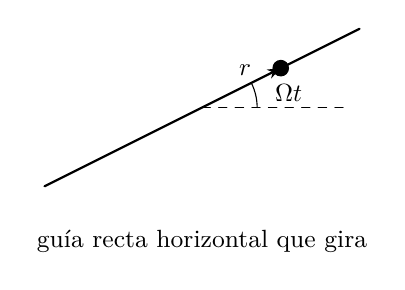
\begin{tikzpicture}[>=Stealth,font=\small,line cap=round,line join=round]
\draw[thick] (-2,-1) -- (2,1);
\fill (1,.5) circle (3pt);
\draw[->,thin,dashed] (0,0) -- (1,0.5) node[pos=0.55,above] {$r$};
\draw (.7,0) arc (0:26.565:.7);
\draw[dashed] (0,0) -- (1.8,0);
\node at (1.1,0.18) {$\Omega t$};
\node at (0,-1.7) {guía recta horizontal que gira};

\end{tikzpicture}
\end{document}
